\documentclass[twocolumn]{article}
\usepackage{multicol}
\usepackage[affil-it]{authblk}
\usepackage{amsmath}
\usepackage{tcolorbox}
\makeatletter
\newcommand{\vo}{\vec{o}\@ifnextchar{^}{\,}{}}
\makeatother
\usepackage{graphicx}
\setlength{\parindent}{4mm}
\setlength{\parskip}{0mm}
\renewcommand{\baselinestretch}{1.3}
\begin{document}
%##############################################
%TITLE PAGE
\title{PHYSICS 660: Radioactive Decay of Nuclei A and B}
\author{Andrew Crossman}
\affil{Department of Physics and Astronomy, University of Delaware}
\date{February, 18th 2019}
\maketitle
\newpage

\twocolumn[
\begin{@twocolumnfalse}
%###############################################
%ABSTRACT
\begin{abstract}
This article will discuss the behavior of the radioactive decay of two types of nuclei: $A$ and $B$ with respective populations $N_a(t)$ and $N_b(t)$. These two populations will be analyzed over time in two different systems: $(i)$ when $A$ decays into $B$ and then $B$ decays, and $(ii)$ when $A$ decays into $B$ then $B$ decays into $A$. The stabilities of both systems will be explored as well as the accuracy of their respective numeric solutions in comparison to their analytic solutions. In conclusion we will find that both systems numeric solutions closely follow their analytic counterparts - with the exception of the first few initial data points. The respective decay constants $\tau_a$ and $\tau_b$ for system $(i)$ will also be shown to greatly affect the stability of the system. In the case that $\tau_a<\tau_b$ the population of $B$ will be shown to surpass that of $A$ quite quickly and remain greater until they both decay to zero. In contrast, when $\tau_a>\tau_b$ the population of $B$ will be revealed to never surpass that of $A$ until all of $A$ decays, thus leaving a handful of $B$ nuclei until they also decay. In the case that $\tau_a=\tau_b=\tau$ we will find that the populations are exactly equal when $t=\frac{195\tau}{200}$, after-which population $B$ will remain greater until they both decay to zero. For system $(ii)$ we will find that as $t\to\infty$ a steady state emerges between the two populations, where the population of $B$ is twice that of population $A$. Before this steady state appears though, we will discern that population $A$ dramatically decreases, consequentially increasing population $B$. The trends of these populations will then be shown to intersect at $t=\frac{2\tau}{3}ln\left(4\right)$ before gradually evolving into resonance.
\end{abstract}
\vspace{5mm}
\end{@twocolumnfalse}
]
%###############################################
%INTRODUCTION
\section{Introduction to Radioactive Decay} 
\hspace{\parindent} Radioactive Decay was first observed by the French Scientist, Henri Becquerel in 1896. Very much an accidental discovery, Henri was experimenting with phosphorescent materials when he noticed that one of his work station's photographic plates had experienced blackening despite its encasing. Upon further inspection, Henri came to realize that the blackening had been solely caused by his samples of uranium and had nothing to do with the phosphorescence. Dubbing this radioactivity "Becquerel Rays," this new form of radiation was initially thought to be similar to the recently discovered X-rays. However, additional experimentation by the scientific community showed that this form of radioactivity was significantly different. Most notably, radioactive decay was shown to occur only as a property of the nucleus of an atom, whereas radiation (such as X-rays) was known to occur as a byproduct of many processes. Eventually, experiments conducted by Rutherford and his student Fredrick Soddy determined that all elements decayed in the same exponential form,
$$N(t)=N_oe^{\lambda t}$$
- another distinction from general radiation - and that many decaying processes also caused a transmutation of the material to a new one. These findings by Henri, Rutherford, and many other scientists of the age sparked a search for other elements with radioactive decay and their total radioactivity. Perhaps the most important of all of these elements would come to be radium. Discovered by Marie and Pierre Curie, their research on radium revealed its potential as a treatment not only for cancer, but as a means of creating nuclear energy. Naturally then, understanding radioactive decay and its properties is a very valuable asset to the general advancement of humanity.

Keeping in the spirit of such advancement, this study of radioactive decay aims to observe two simulated systems composed of two different nuclei: nuclei $A$ and nuclei $B$. The first system will simulate type $A$ nuclei decaying into type $B$ nuclei, and then type $B$ nuclei decaying again. We will track their respective populations as they decay and determine how the stability of their system is affected as we alter their decay constants. In the second simulated system we will likewise have the type $A$ nuclei decay into type $B$ nuclei, but now have the type $B$ nuclei decay into type $A$ again. This second simulation - some may notice - is not "strictly" a decaying model because of its cyclic nature. Never-the-less, we will track the respective type $A$ and $B$ populations, and once again see how the stability of the system is affected as a function of altering its decay constants.
%##############################################
%
\section{Methodology}
\hspace{\parindent} Our two systems $(i)$ and $(ii)$ will be evaluated using both a analytic and numeric approach. The analytic approach will be achieved using the "pen and paper" method where we will solve the respective decay equations for both types of nuclei directly. The numeric approach will be achieved by means of the Euler Method, where we will find approximations to the analytic solutions in the form: $$N_u(t+\delta t)=N_u(t)+\frac{dN_u(t)}{dt}\delta t$$Using graphic data based off of our analytic and numeric calculations we will then see how changing $\tau_a$ and $\tau_b$ in the following cases:
	\begin{align}
	\tau_a&>\tau_b\\
	\tau_a&<\tau_b\\
	\tau_a&=\tau_b
	\end{align}
affects the stability of the type $A$ and $B$ populations over time in system $(i)$. In system $(ii)$ we will verify that our numeric and analytic results verify that the system will eventually reach a steady state where the type $A$ and $B$ populations remain constant. We will also compare the accuracy of the analytic and numeric solutions of both models to determine whether or not the Euler method is an effective means of getting "reasonable" approximations or not.
\section{System $(i)$ Solution}
\hspace{\parindent} As mentioned before, system $(i)$ is composed of two different nuclei $A$ and $B$, in which type $A$ nuclei decay into type $B$ nuclei followed by type $B$ nuclei decaying again. This dual decay can be described by the following differential equations:
	\begin{align}
	\frac{dN_a}{dt}&=-\frac{N_a}{\tau_a} \\
	\frac{dN_b}{dt}&=\frac{N_a}{\tau_a}-\frac{N_b}{\tau_b}
	\end{align}
where $\tau_a$ and $\tau_b$ are the respective decay time constants for each type of nuclei. The initial conditions for this system are also given as $N_a(0)=200$ and $N_b(0)=5$ for $t=0$. 
\subsection{Analytic Solution to $N_a(t)$}
\hspace{\parindent} Equation $(1)$ can be used to directly solve $N_a(t)$ by using elementary methods of solving Ordinary Differential Equations. Hence,
	\begin{align}
	\frac{dN_a}{dt}&=-\frac{N_a}{\tau_a}\\
	\frac{1}{N_a}dN_a&=-\frac{1}{\tau_a}dt\\
	\int_{}{}\frac{1}{N_a}dN_a&=-\int_{}{}\frac{1}{\tau_a}dt\\
	\ln(N_a)&=\frac{-t}{\tau_a}+C\\
%	N_a(t)&=e^{\frac{-t}{\tau_a}+C}\\
%	N_a(t)&=e^{C}e^{\frac{-t}{\tau_a}}\\
	N_a(t)&=Ke^{\frac{-t}{\tau_a}}
	\end{align}
Now that we have isolated $N_a(t)$ all we need to do is solve for the initial conditions (i.e. $N_a(0)=200$).
	\begin{align}
	N_a(0)=200=Ke^{\frac{-0}{\tau_a}}\\
	200=K
	\end{align}
Hence, our analytic solution to $N_a(t)$ is:
	\begin{align}
	N_a(t)=200e^{\frac{-t}{\tau_a}}
	\end{align}
\subsection{Analytic Solution to $N_b(t)$}
\hspace{\parindent} Now that we have $N_a(t)$ we can solve equation $(5)$ for $N_b(t)$. Notice that equation $(5)$ is in normal linear form and can consequently be solved by using an integrating factor. This integrating factor is by definition $\mu(t)=e^{\int_{}{}\rho(t)dt}$, where $\rho(t)$ is taken from the form $\frac{dy}{dt}+\rho(t)y=q(t)$. Hence our integration factor is, 
	\begin{align}
	\frac{dN_b}{dt}+\frac{N_b}{\tau_b}=\frac{N_a}{\tau_a}\\
	\rho(t)=\frac{1}{\tau_b}, y=N_b\\
	\mu(t)=e^{\int_{}{}\frac{1}{\tau_b}dt}\\
	\mu(t)=e^{\frac{t}{\tau_b}}
	\end{align}
Applying this integrating factor and substituting in our solution for $N_a(t)$ we find that...
	\begin{align}
	e^{\frac{t}{\tau_b}}\frac{dN_b}{dt}+e^{\frac{t}{\tau_b}}\frac{N_b}{\tau_b}&=e^{\frac{t}{\tau_b}}\frac{Na}{\tau_a}\\
	\frac{d}{dt}\left[e^{\frac{t}{\tau_b}}N_b\right]&=e^{\frac{t}{\tau_b}}\frac{N_a}{\tau_a}\\
	\int_{}{}\frac{d}{dt}\left[e^{\frac{t}{\tau_b}}N_b\right]dt&=\int_{}{}e^{\frac{t}{\tau_b}}\frac{N_a}{\tau_a}dt\\
	e^{\frac{t}{\tau_b}}N_b&=\int_{}{}e^{\frac{t}{\tau_b}}\frac{200e^{\frac{-t}{\tau_a}}}{\tau_a}dt\\
	e^{\frac{t}{\tau_b}}N_b&=\frac{200}{\tau_a}\frac{e^{t\left(\frac{1}{\tau_b}-\frac{1}{\tau_a}\right)}}{\left(\frac{1}{\tau_b}-\frac{1}{\tau_a}\right)}+K\\
	N_b&=\frac{200\tau_b}{\left(\tau_a-\tau_b\right)}e^{\frac{-t}{\tau_a}}+Ke^{\frac{-t}{\tau_b}}	
	\end{align}
Solving for the initial conditions of $Nb(0)=5$ we see that...
	\begin{align}
	N_b(0)=5&=\frac{200\tau_b}{\left(\tau_a-\tau_b\right)}e^{\frac{-0}{\tau_a}}+Ke^{\frac{-0}{\tau_b}}\\
	5&=\frac{200\tau_b}{\left(\tau_a-\tau_b\right)}+K\\
	K&=5-\frac{200\tau_b}{\left(\tau_a-\tau_b\right)}
	\end{align}
Therefore, our solution for $Nb(t)$ is...
	\begin{align}
	N_b(t)=\frac{200\tau_be^{\frac{-t}{\tau_a}}}{\left(\tau_a-\tau_b\right)}+\left(5-\frac{200\tau_b}{\left(\tau_a-\tau_b\right)}\right)e^{\frac{-t}{\tau_b}}
	\end{align}
Upon closer inspection, however, this solution does have a problem. It is undefined when $\tau_a=\tau_b$. Fortunately, solving $N_b(t)$ for this case is still possible if we use a little "trick." Since, we know $\tau_a=\tau_b$ we can simply assign them a new variable $\tau$. Hence the initial ODE for equation $(5)$ becomes...
	\begin{align}
	\frac{dN_b}{dt}=\frac{Na}{\tau}-\frac{Nb}{\tau}
	\end{align}
with a new integrating factor of...
	\begin{align}
	\mu(t)=e^{\frac{t}{\tau	}}
	\end{align}
Following the previous steps outlined in equations $(18)-(27)$ yields a solution of...
	\begin{align}
	N_b(t)=\frac{200te^{\frac{-t}{\tau}}}{\tau}+5e^{\frac{-t}{\tau}}:\tau_a=\tau_b=\tau
	\end{align}
Hence, our solution to $N_b(t)$ is complete. It should be noted at this time, though, that we have been making a big assumption: that $\tau$, $\tau_a$, and $\tau_b$ be greater than zero. In fact this assumption is more than just an assumption, but a factual consequence of the nature of the decay constant. That is to say, that the decay constant must always be $\tau>0$, otherwise there would be no decay in the first place! 
\subsection{Numeric Solutions for $N_a(t)$ and $N_b(t)$}
\hspace{\parindent} Now that we've done the difficult work of solving the analytic equations, all that is left to do for system $(i)$ is setup the numeric equations for $N_a(t)$ and $N_b(t)$. This is naturally much easier to do than with their analytic counterparts - lest we would just use the analytic solution every time! In fact it is as simple as substituting equations $(4)$ and $(5)$ into our Euler method formula. Hence,
	\begin{align}
	N_a(t+\delta t)&=N_a(t)+\frac{dN_a(t)}{dt}\delta t\\
	N_a(t+\delta t)&=N_a(t)+\left(-\frac{N_a}{\tau_a}\right)\delta t\\
	N_a(t+\delta t)&=N_a(t)-\frac{N_a}{\tau_a}\delta t\\
	N_b(t+\delta t)&=N_b(t)+\frac{dN_b(t)}{dt}\delta t\\
	N_b(t+\delta t)&=N_b(t)+\left(\frac{N_a(t)}{\tau_a}-\frac{N_b}{\tau_b}\right)\delta t
	\end{align}	 
where are simplified numeric equations for $N_a(t)$ and $N_b(t)$ are $(33)$ and $(35)$.
\subsection{System $(i)$ Analysis}
\hspace{\parindent} Having finally derived all of the relevant equations, we can produce the pertinent plots of the type $A$ and $B$ populations. Note that in the graphs' legends, $N_a(t)$ and $N_b(t)$ refer to the numeric solutions  where as $exact N_a(t)$ and $exact N_b(t)$ refer to the analytic solutions at $time=\frac{t}{\tau_a}$. It should also be noted that $\delta t$ for each graph is .25 which equates to four data points for each one unit of time as indicated by the x-axis.

\begin{figure}[h]
\caption{$\tau_a = \tau_b = 1$}
\centering
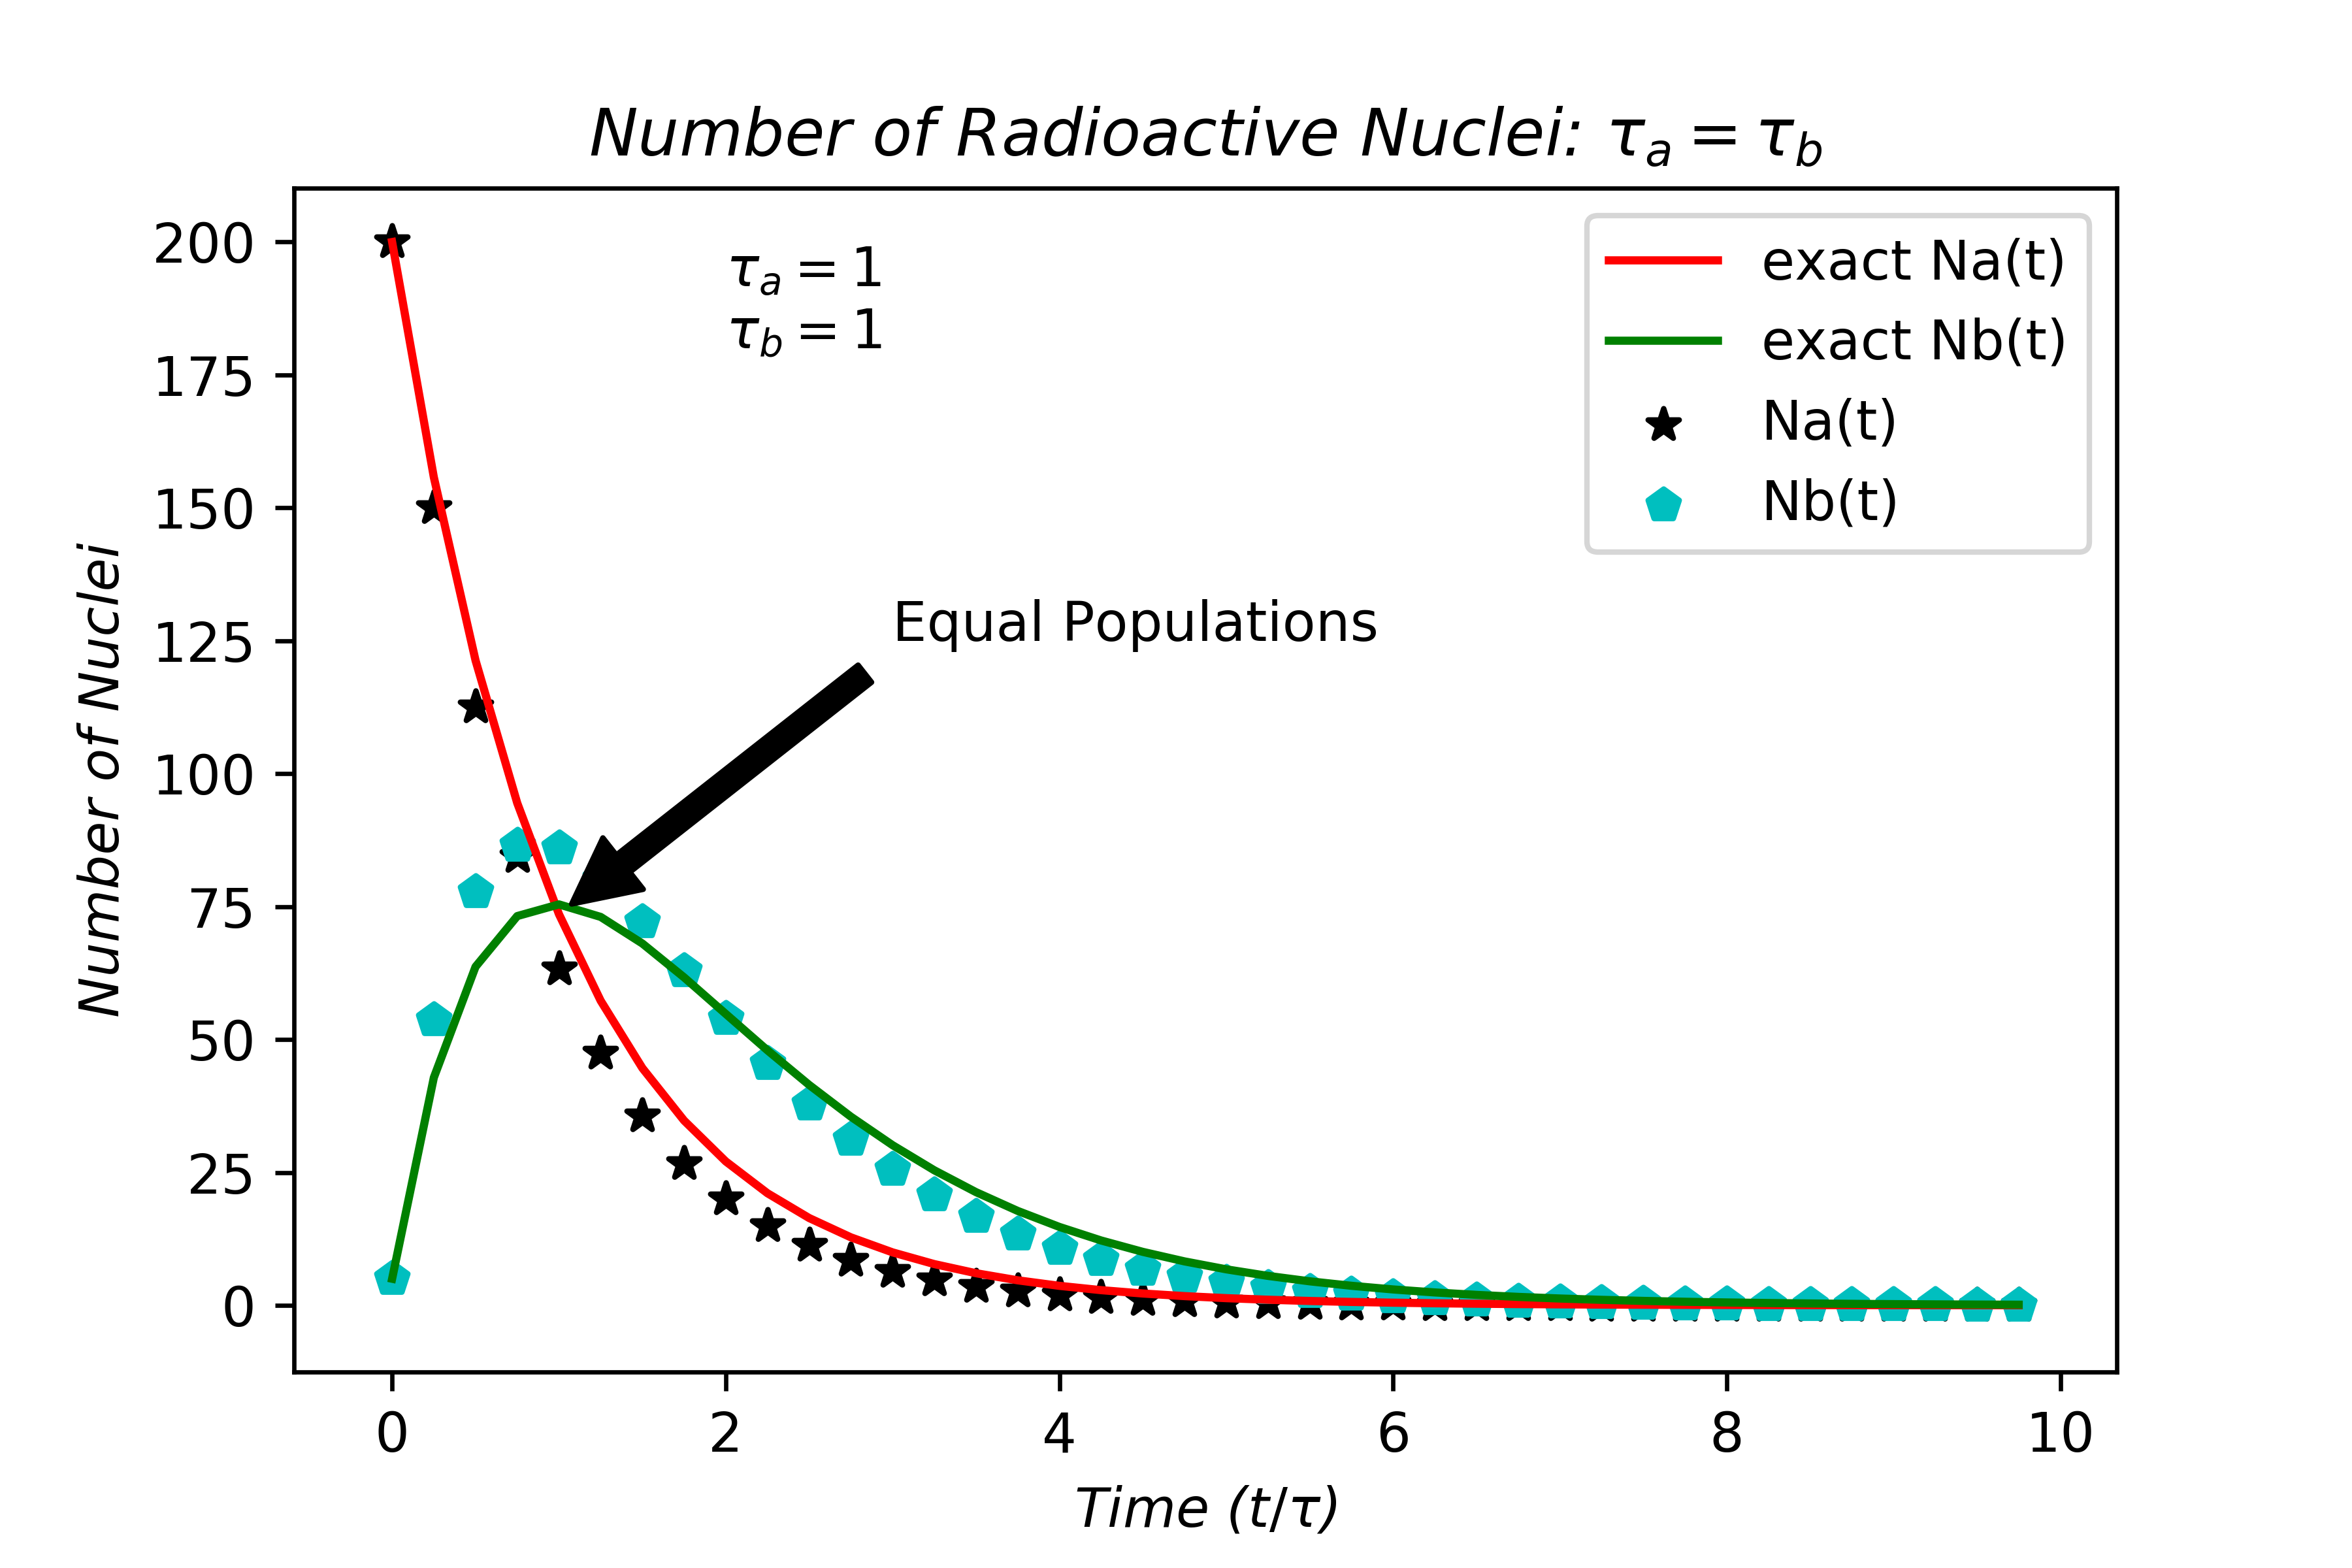
\includegraphics[scale=.6]{Radioactive_DecayAequalB}
\end{figure}

In our first plot (Figure 1), $\tau_a = \tau_b = 1$. The numeric solutions are quite accurate, although still clearly in disagreement from the analytic solutions by a not insignificant percentage up until $time \approx 3$, after-which the difference is almost impossible to distinguish. At $time=\frac{195\tau}{200}$ we can also see that both populations contain the exact same amount of nuclei. This time at which the two populations are equal makes sense from both a physical and mathematical sense as well. Physically, we know that at $time=1$ population $A$ should be at $\frac{200}{e}$ of its initial value according to the rules radioactive decay. We also know that these decayed nuclei form type $B$ nuclei which then also decay according to the same rate. Hence, it is not surprising that around $time=1$ in a $time = \frac{t}{\tau}$ scale that the two populations would meet. Mathematically we can see this as:
	\begin{align}
	N_a(t)&=N_b(t)\\
	200e^{\frac{-t}{\tau}}&=\frac{200te{\frac{-t}{tau}}}{\tau}+5e^{\frac{-t}{\tau}}\\
	t&=\left(200-5\right)\frac{tau}{200}\\
	t&=\frac{195\tau}{200}
	\end{align}
It is also of interest to note that after this time that the type $B$ population remains greater than the type $A$ population until they both decay to 0.

\begin{figure}[h]
\caption{$\tau_a = 1$, $\tau_b = .2$}
\centering
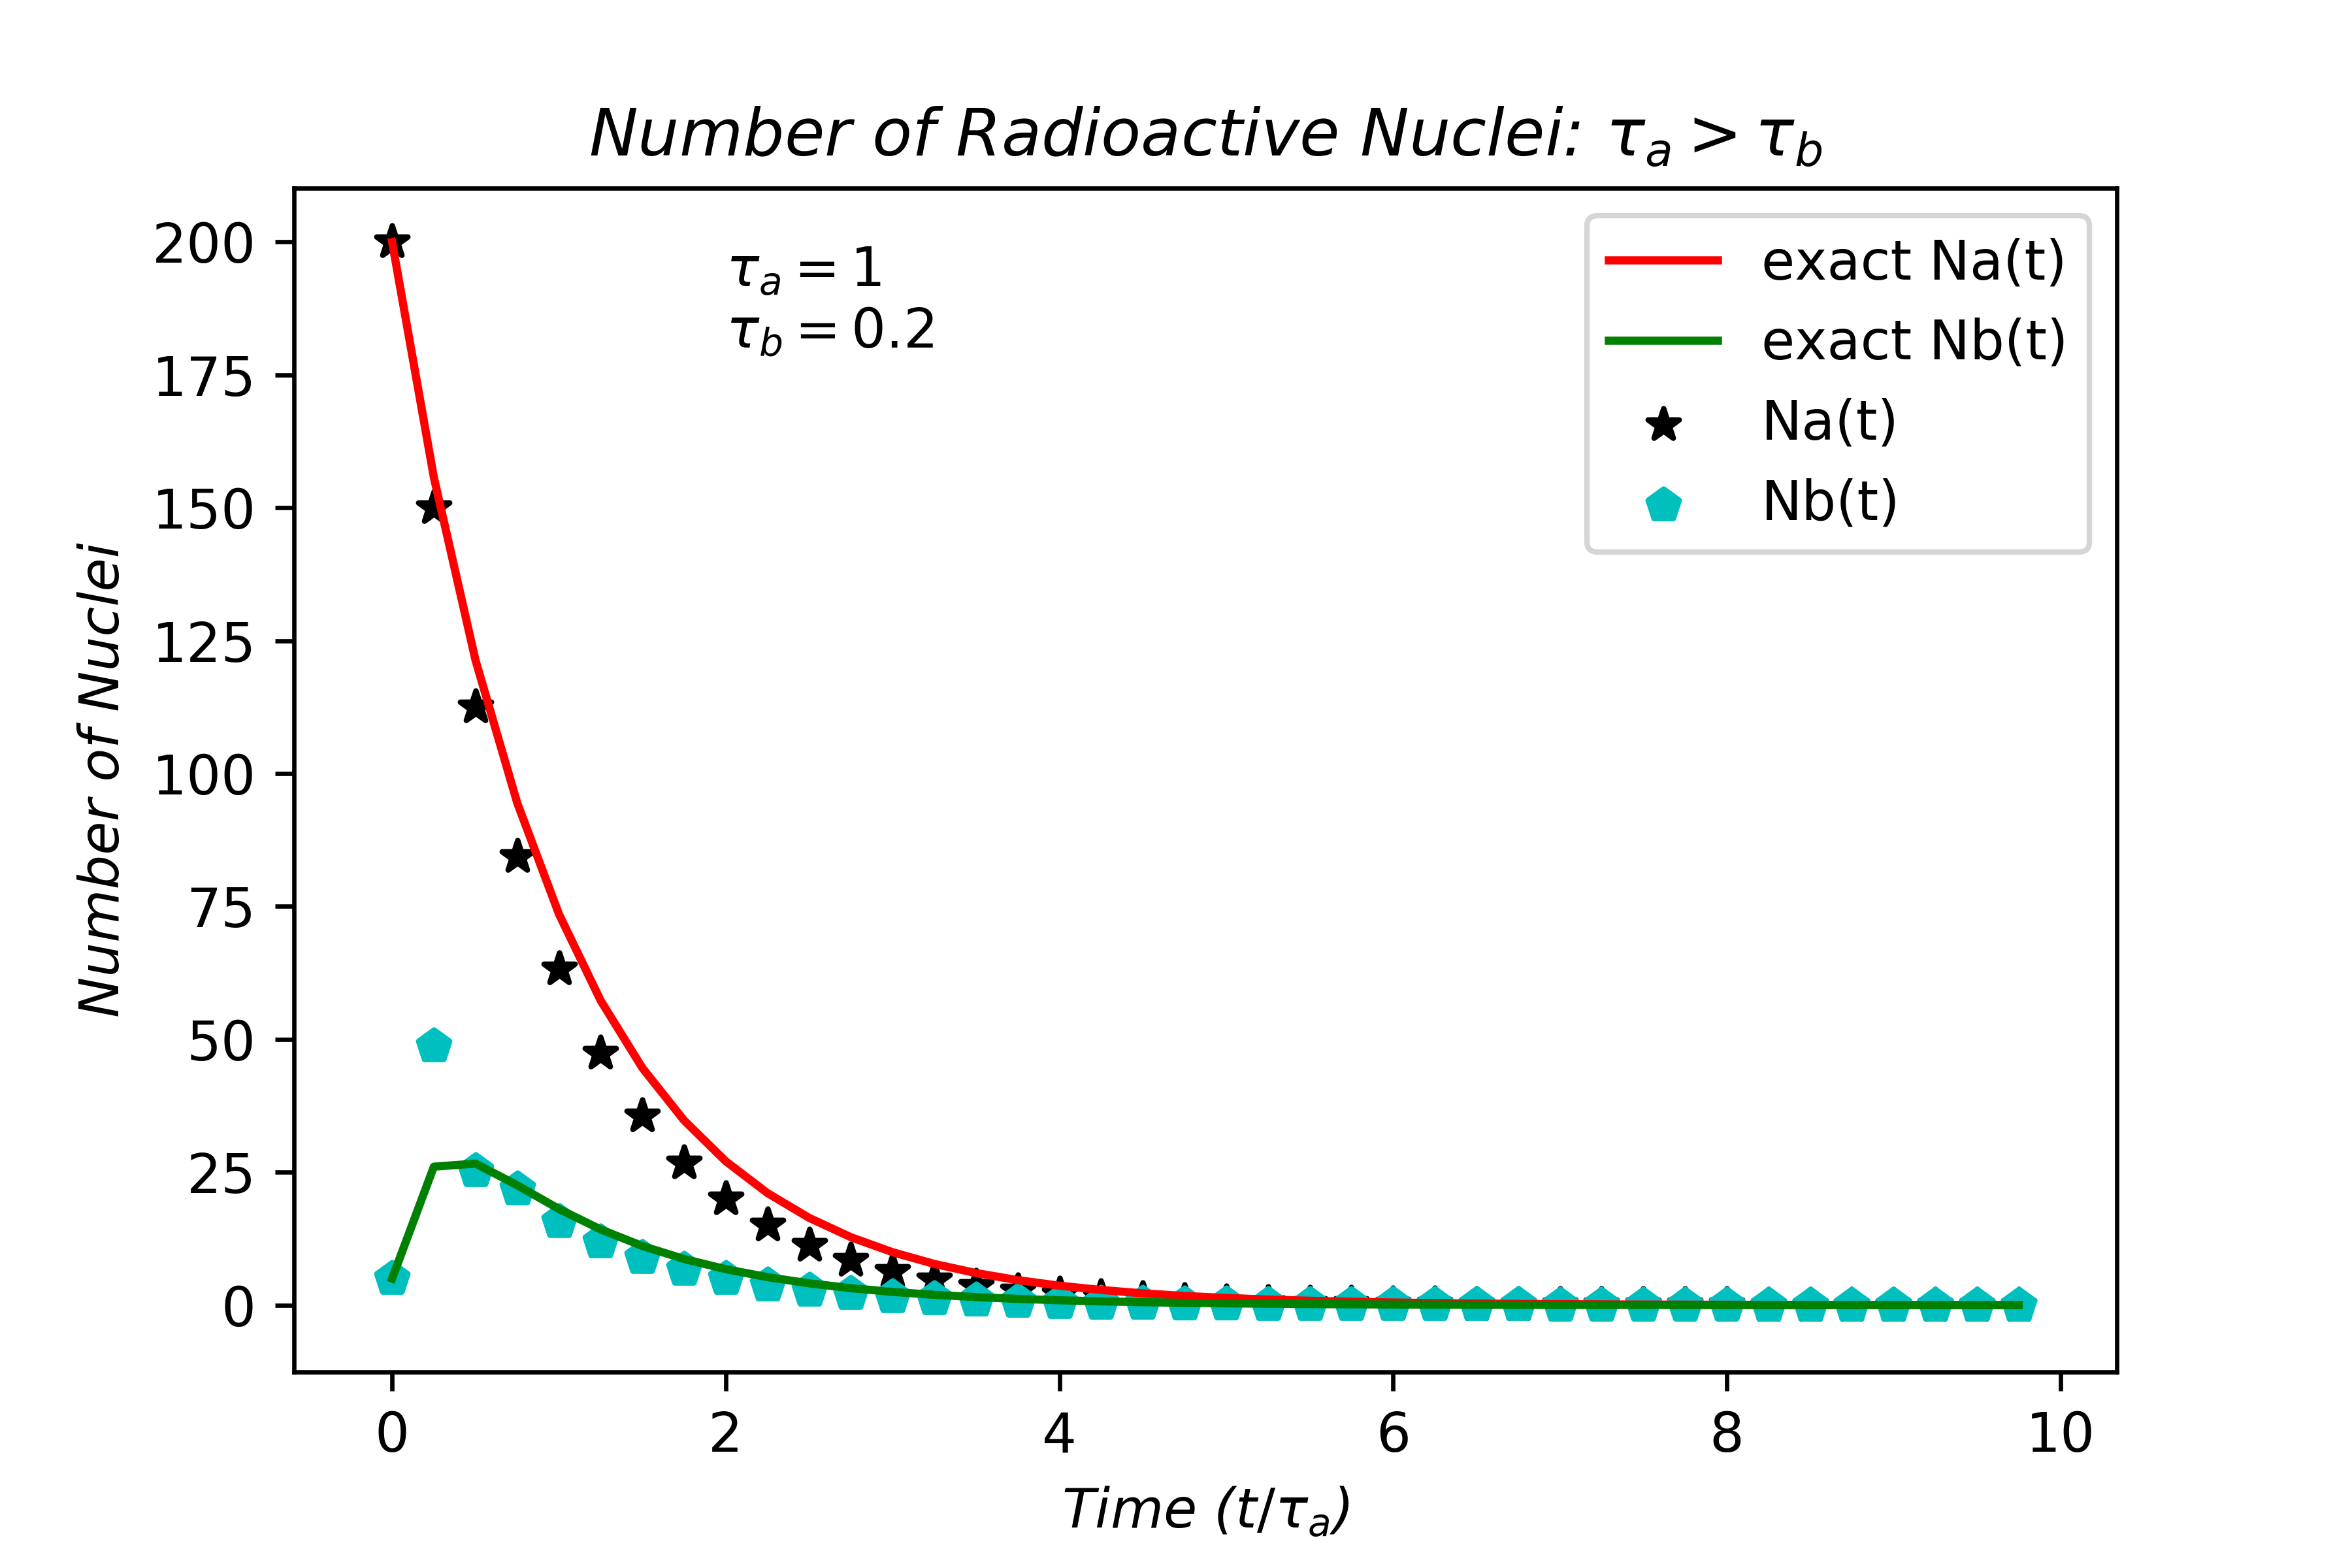
\includegraphics[scale=.6]{Radioactive_DecayAgreaterthanB}
\end{figure}
In our second plot (Figure 2), $\tau_a=1$ and $\tau_b=.2$. Again, the numeric solutions appear to  agree very well with the analytic solutions, with the exception of the first initial approximations for $N_b(t)$ and the approximations between times $1-3$ for $N_a(t)$. Aside from this, a big distinction that should be noted here is in the behavior of the type $A$ and $B$ populations. In Figure 1, we discerned that at $time=\frac{195\tau}{200}$ the two populations were equal; however, there exists no such time in which this is true under the condition that $\tau_a>\tau_b$. Thinking about this from a physical perspective makes a lot of sense, too. Consider that because $\tau_a$ is larger than $\tau_b$, it requires a longer period of time for type $A$ nuclei to decay than it does type $B$ nuclei. Then also consider that the initial conditions of the system are $N_a(0)=200$ and $N_b(0)=5$. Hence, type $A$ nuclei start off with a larger population and also decay more slowly than its type $B$ counterpart. In this way it is very easy to justify that the type $A$ population should most certainly be larger than the type $B$ population for all time (or at least until the last type $A$ nuclei decays into a $B$ nuclei).

\begin{figure}[h]
\caption{$\tau_a = 1$, $\tau_b = 5$}
\centering
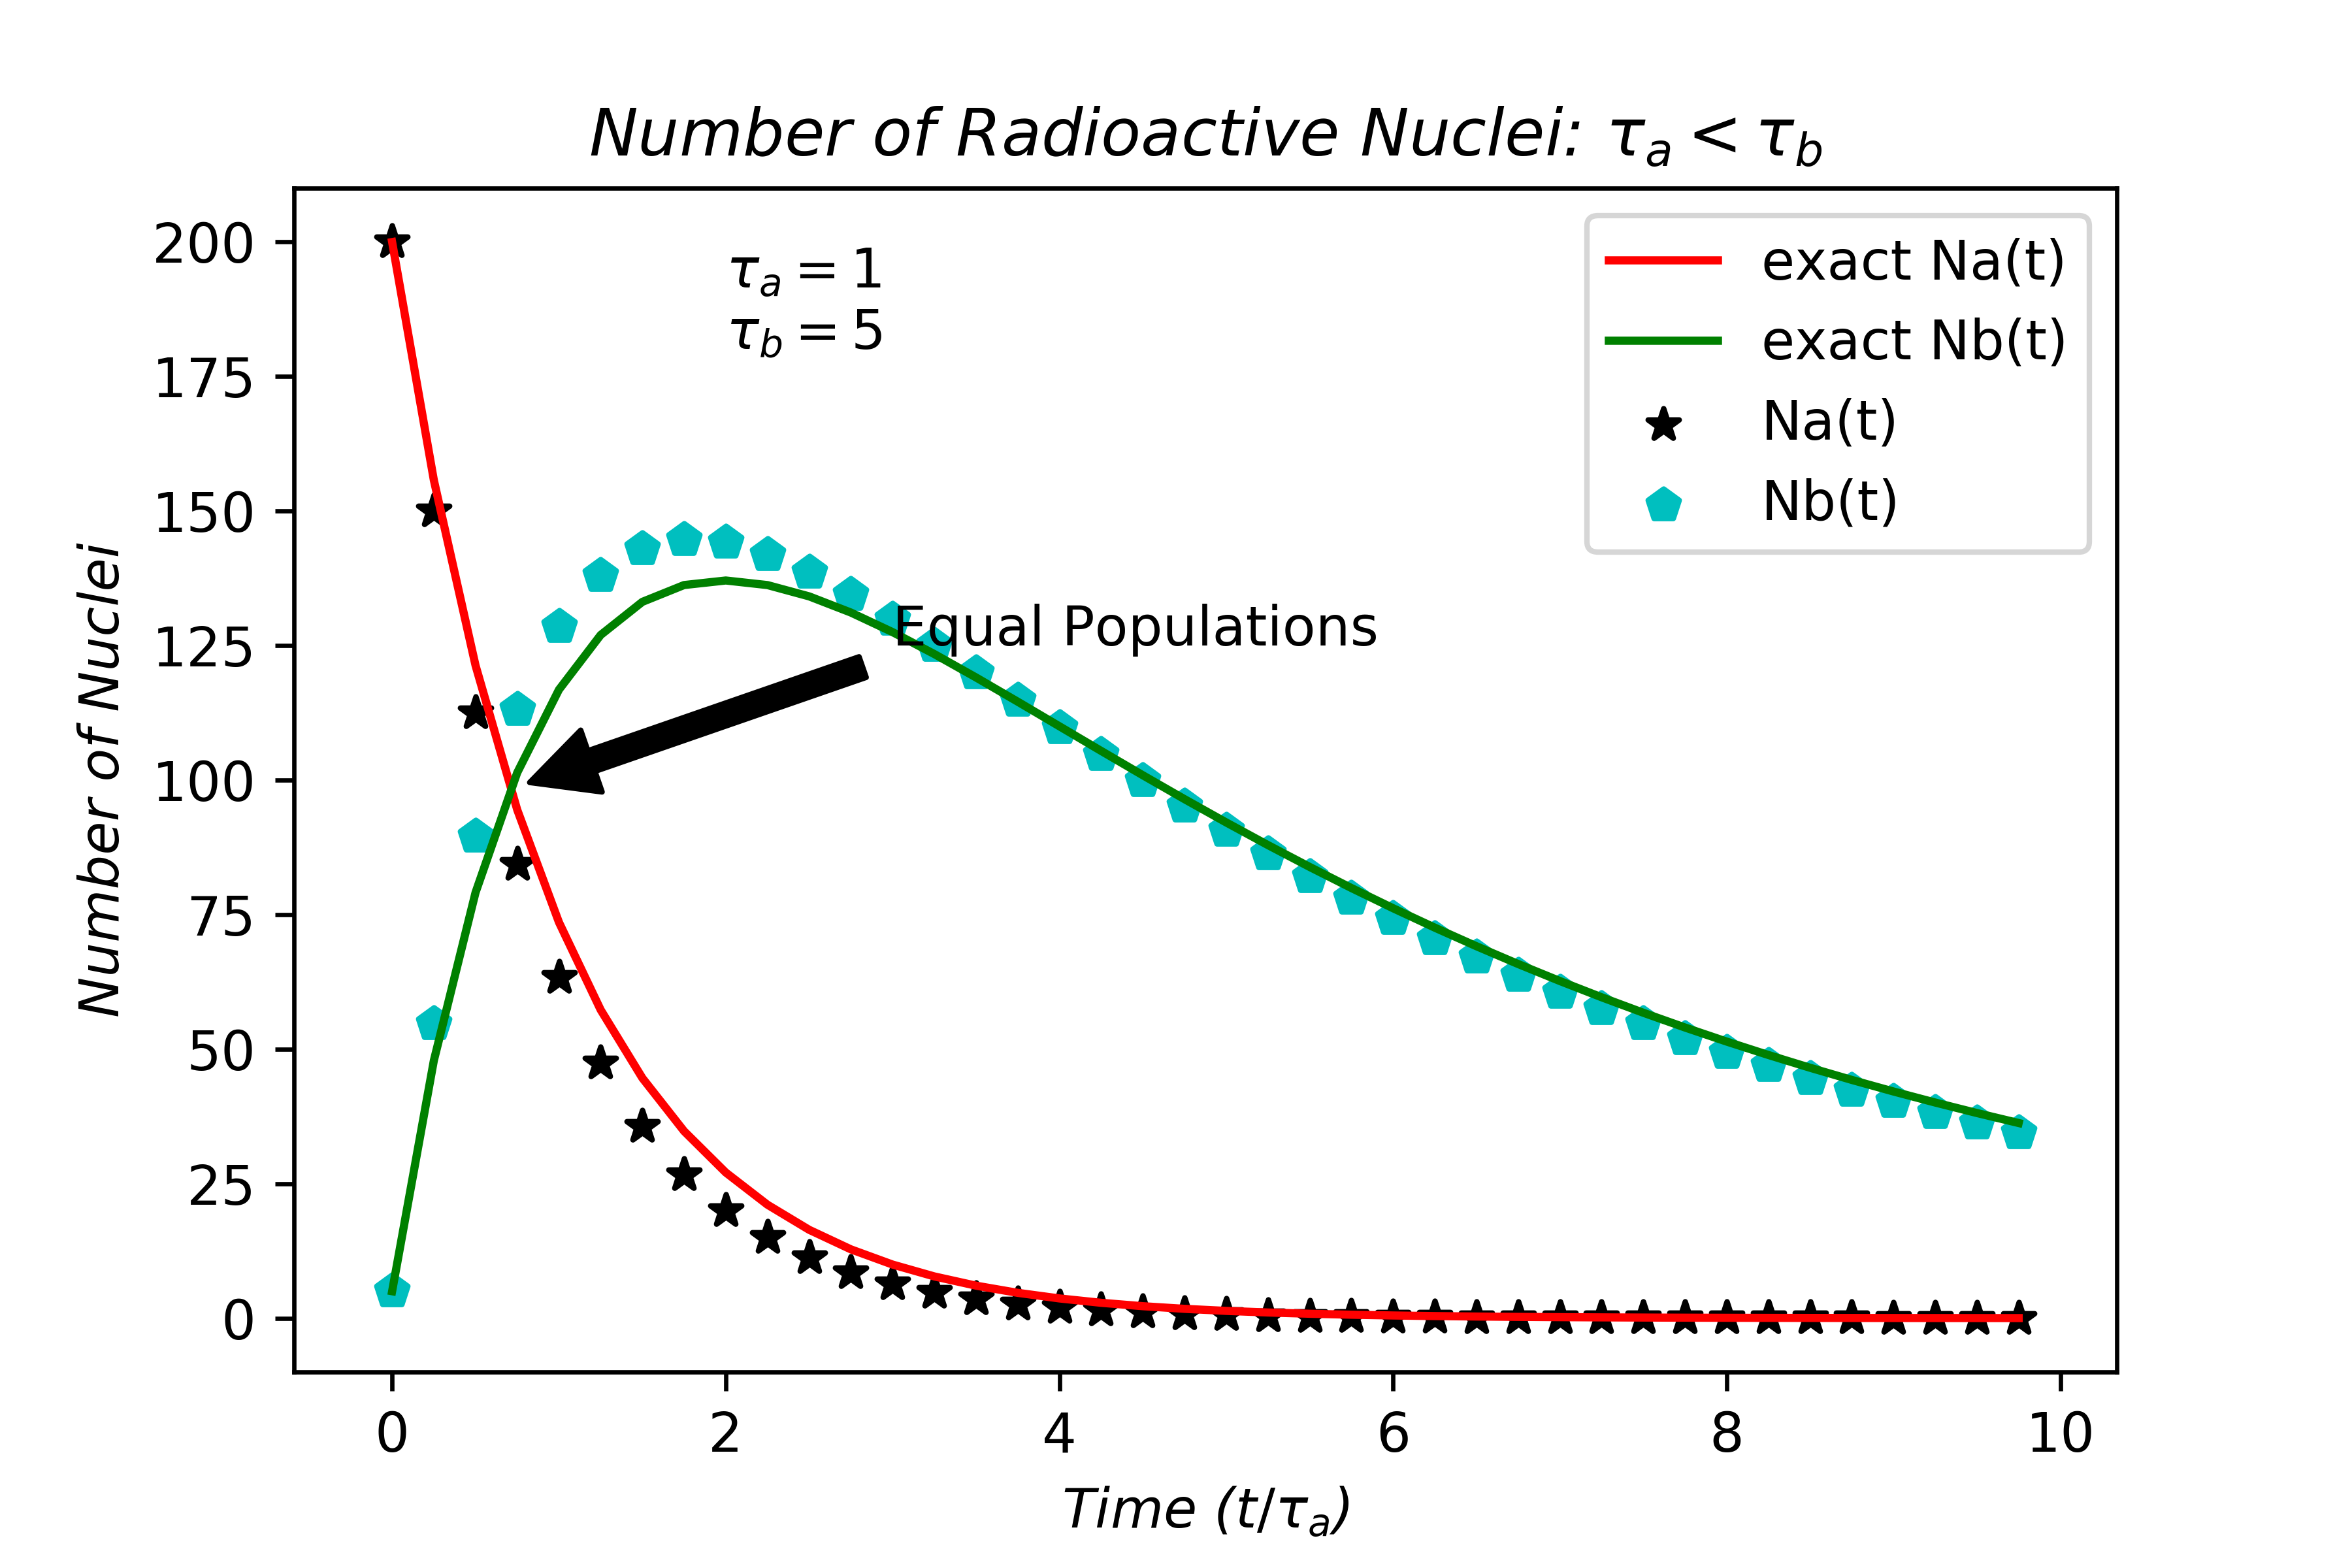
\includegraphics[scale=.6]{Radioactive_DecayAlessthanB}
\end{figure}
Our final graph (Figure 3), has decay constants $\tau_a=1$ and $\tau_b=5$. Clearly then, $\tau_a<\tau_b$ and so as the shrewd scientists that we are, we should expect a different behavior than the previous two conditions we've observed. This statement is at the very least partially correct. If we once again, look at Figure 1. we can see that there are some very distinct similarities between it and Figure 3. Namely, they both have a time at which the two populations are equal to one another, after-which population $B$ remains greater than $A$. From a physical sense, we should expect this occurrence because the decay constant for the type $B$ nuclei is larger than the type $A$ nuclei, and so over time a large portion of the type $A$ nuclei will decay into the type $B$ nuclei, which will then take a long time in comparison to decay. Its akin to a funnel, where the contents going into the funnel are the decayed $A$ nuclei (now type $B$) and are all being "bottle-necked" since it takes a long time for them to decay again (go through the funnel). Mathematically, the time at which this happens can be calculated by setting equations $(13)$ and $(27)$ equal to one another and then solving for $t$.
	\begin{align}
	N_a(t)&=N_b(t)\\
	200e^{\frac{-t}{\tau_a}}&=\frac{200\tau_b}{\tau_a-\tau_b}e^{\frac{-t}{\tau_a}}+\left(5-\frac{200\tau_b}{\tau_a-\tau_b}\right)e^{\frac{-t}{\tau_b}}\\
	e^{t\left(\frac{1}{\tau_a}-\frac{1}{\tau_b}\right)}&=\frac{200-\frac{200\tau_b}{\tau_a-\tau_b}}{5-\frac{200\tau_b}{\tau_a-\tau_b}}\\
	t&=\frac{1}{\frac{1}{\tau_a}-\frac{1}{\tau_b}}ln\left[\frac{200-\frac{200\tau_b}{\tau_a-\tau_b}}{5-\frac{200\tau_b}{\tau_a-\tau_b}}\right]	
	\end{align}
Although it is certainly an intimidating expression, its derivation is quite simple. On a final note, it is quite important to recognize that like our previous plots our numeric solutions overshoot our analytic ones when the populations are increasing and undershoot our analytic ones when decreasing. This effect minimizes as $t\to\infty$ and like the other Figures becomes near indiscernible. 
\section{System $(ii)$ Solution}
\hspace{\parindent} Similarly to system $(i)$, system $(ii)$ is composed of the same two nuclei we have discussing: type $A$ and type $B$. These "decays" are described by the equations:
	\begin{align}
	\frac{dN_a}{dt}&=\frac{N_b}{2\tau}-\frac{N_a}{\tau}\\
	\frac{dN_b}{dt}&=\frac{N_a}{\tau}-\frac{N_b}{2\tau}
	\end{align}
where $\tau$ is the singular decay constant. The initial conditions are also given as $N_a(0)=150$ and $N_b(0)=0$. I quoted "decays" earlier because unlike the previous system, the type $B$ nuclei will now decay into a type $A$ nuclei. This characteristic of the system makes it not a decaying one in the true sense and, hence the quotations. 
\subsection{Simultaneous Analytic Solutions}
\hspace{\parindent} For the previous system, we first solved $N_a(t)$ and then $N_b(t)$ in that order using substitution. In this system's case we can not do that; however, because equations $(44)$ and $(45)$ are convoluted with one another. Hence, a different method is necessary. Let us try setting up the problem as a system of matrices:
	\begin{equation}
	x'=\left(\frac{N_a'}{N_b'}\right)=Ax=
	\frac{1}{2\tau}\left(\begin{array}{cc} -2 & 1\\ 2 & -1 \end{array}\right)
	\left(\begin{array}{c} N_a\\ N_b\end{array}\right)
	\end{equation}
	\begin{equation}
	\left|A-\lambda I\right|=0=
	\frac{1}{2\tau}\left(\begin{array}{cc} -2-\lambda & 1\\ 2 & -1-\lambda \end{array}\right)
	\end{equation}
	\begin{equation}
	0=\frac{\lambda}{\tau}+\frac{\lambda}{2\tau}+\lambda^2 
	\end{equation}
	\begin{equation}
	0=\lambda\left(\frac{3}{2\tau}+\lambda\right)
	\end{equation}
	\begin{equation}
	\lambda_0=0,\lambda_1=-\frac{3}{2\tau}
	\end{equation}
Now that we have our eigenvalues, let us use them in the equation $\left(A-\lambda I\right)\vec{v}=0$ to determine our eigenvectors. Hence...
\\case One: $\lambda = \lambda_0 = 0$
	\begin{equation}
	\left(A-\lambda_0 I\right)\vec{v_0}=\frac{1}{2\tau}\left(\begin{array}{cc} -2 & 1\\ 2 & -1\end{array}	\right)\left(\begin{array}{c} v_1\\ v_2 \end{array}\right)=0
	\end{equation}
Simplifying the matrix we find that...
	\begin{equation}
	2v_1=v_2 \implies \vec{v_0}=\left(\begin{array}{cc} 1 & 2\end{array}\right)^{T}
	\end{equation}
\\case Two: $\lambda = \lambda_1 = -\frac{3}{2\tau}$
	\begin{equation}
	\left(A-\lambda_1 I\right)\vec{v_1}=\frac{1}{2\tau}\left(\begin{array}{cc} 1 & 1\\ 2 & 2\end{array}	\right)\left(\begin{array}{c} v_1\\ v_2 \end{array}\right)=0
	\end{equation}
Again simplifying the matrix we find that...
	\begin{equation}
	v_1=-v_2 \implies \vec{v_1}=\left(\begin{array}{cc} 1 & -1\end{array}\right)^{T}
	\end{equation}
Now that we have our two eigenvectors we can substitute them into the general equation:
	\begin{equation}
	\vec{x}(t)=K_0\vec{v_0}e^{\lambda_0 t} + K_1\vec{v_1}e^{\lambda_1 t}
	\end{equation}
	\begin{equation}
	\vec{x}(t)=K_0\left(\begin{array}{c} 1\\ 2\end{array}\right)+K_1\left(\begin{array}{c} 1\\ -1\end{array}\right)e^{-\frac{3t}{2\tau}}
	\end{equation}
Applying our initial conditions to solve for $K_0$ and $K_1$ we find that...
	\begin{equation}
	\left(\begin{array}{c} N_a(t)\\ N_b(t)\end{array}\right) = \left(\begin{array}{c} K_0+K_1e^{-\frac{3t}{2\tau}}\\ 2K_0-K_1e^{-\frac{3t}{2\tau}}\end{array}\right)
	\end{equation}	
	\begin{equation}
	\left(\begin{array}{c} N_a(0)\\ N_b(0)\end{array}\right)=\left(\begin{array}{c} 150\\ 0\end{array}\right) = \left(\begin{array}{c} K_0+K_1\\ 2K_0-K_1\end{array}\right)
	\end{equation}
Simply solving for $K_0$ and $K_1$ now, we obtain...
	\begin{equation}
	0=2K_0-K_1 \implies K_1=2K_0\\
	\end{equation}
	\begin{equation}
	150=3K_0 \implies K_0=50 \implies K_1=100
	\end{equation}
Hence, we find that our analytic solutions to $N_a(t)$ and $N_b(t)$ are:
	\begin{equation}
	\left(\begin{array}{c} N_a(t)\\ N_b(t)\end{array}\right) = \left(\begin{array}{c} 50+100e^{-\frac{3t}{2\tau}}\\ 100-100e^{-\frac{3t}{2\tau}}\end{array}\right)
	\end{equation}
\subsection{Numeric Solutions}
\hspace{\parindent} Now that we've gone through the effort of rigorously calculating the analytic solution, we just need to formulate our numeric solutions. We will again use the Euler method that we applied in system $(i)$; only this time we will apply the method to equations $(44)$ and $(45)$. Hence, our numeric solutions are:
	\begin{align}
	N_a(t+\delta t)&=N_a(t)+\frac{dN_a(t)}{dt}\delta t\\
	N_a(t+\delta t)&=N_a(t)+\left(\frac{N_b(t)}{2\tau}-\frac{N_a(t)}{\tau}\right)\delta t\\
	N_a(t+\delta t)&=50+100e^{-\frac{3t}{2\tau}}+\frac{150}{\tau}e^{-\frac{3t}{2\tau}}\delta t\\
	N_b(t+\delta t)&=N_b(t)+\frac{dN_b(t)}{dt}\delta t\\
	N_b(t+\delta t)&=N_b(t)+\left(\frac{N_a(t)}{\tau}-\frac{N_b(t)}{2\tau}\right)\delta t\\
	N_b(t+\delta t)&=100-100e^{-\frac{3t}{2\tau}}-\frac{150}{\tau}e^{-\frac{3t}{2\tau}}\delta t
	\end{align}
where equations $(64)$ and $(67)$ represent our simplified solutions for $N_a(t)$ and $N_b(t)$.
\subsection{System $(ii)$ Analysis}
\hspace{\parindent} Now that we have derived all of the relevant equations, we can finally plot the behavior of the type $A$ and $B$ populations. Note that - as before - in the graph's legend $N_a(t)$ and $N_b(t)$ refer to the numeric solutions where as $exactN_a(t)$ and $exactN_b(t)$ refer to the analytic solutions at $time=\frac{t}{\tau}$. Also recall that $\delta t$ for the plot is .25, which equates to four data points per unit of time as indicated by the x-axis.

\begin{figure}[h]
\caption{$\tau = 1$}
\centering
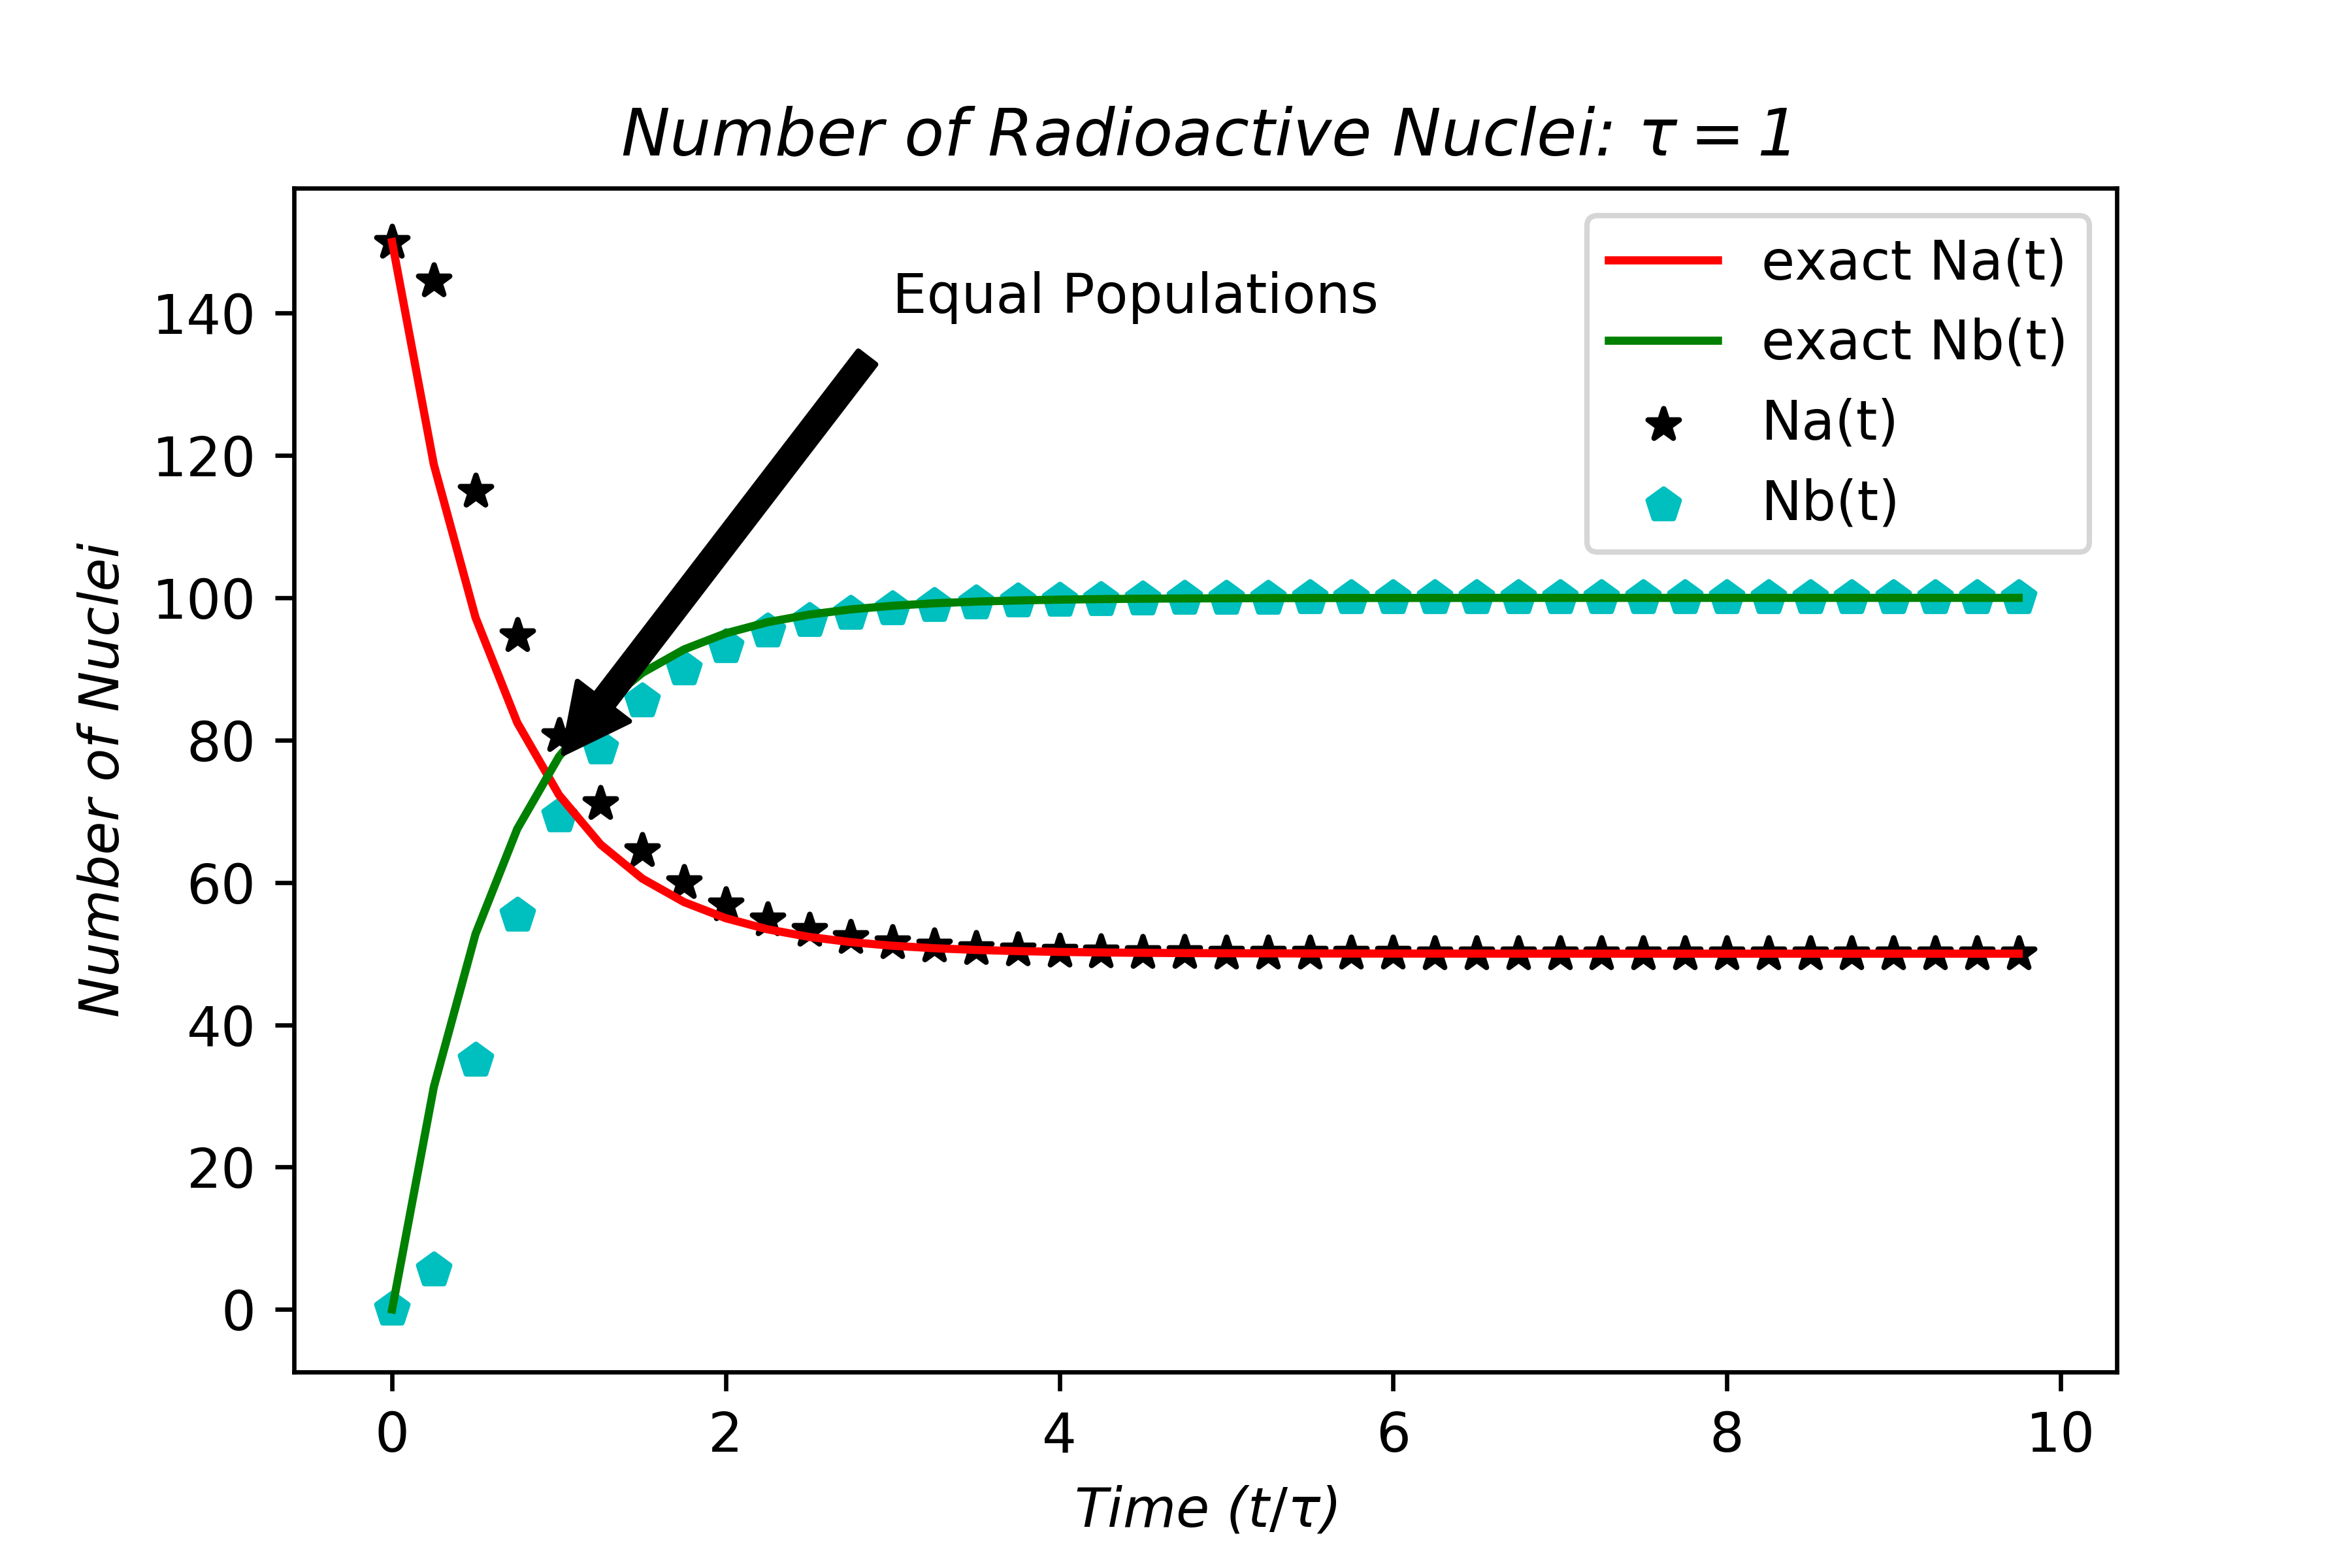
\includegraphics[scale=.6]{Radioactive_DecayPart2}
\end{figure}
Firstly, unlike our other plots from system $(i)$ here we see that our numeric results actually undershoot the analytic ones when the populations are increasing and overshoot them when decreasing. Aside from this, the numeric results act in much the same way as previously - remaining more inaccurate for the first initial data points, and then as time increases, becoming nearly indistinguishable. Secondly, there exists a time at which both populations are equal to one another. Physically, we can explain this phenomena by inspecting the derivatives of $N_a(t)$ and $N_b(t)$ expressed in equations $(44)-(45)$. These two equations describe the rate of change of the $A$ and $B$ populations as $\left|\frac{N_a}{\tau}-\frac{N_b}{2\tau}\right|$. This magnitude reveals that it would take a population of twice $N_a$'s size for $N_b$ to have the same affect on the rate of change due to the additional factor of $\frac{1}{2}$ encompassing $N_b$. Now if we consider that population $A$ starts with an initial value of $150$ compared to population $B$'s initial value of $0$, it should come as no surprise that population $A$ quickly declines where as population $B$ quickly rises thus intersecting. We can describe the time of this intersection by setting $N_a(t)=N_b(t)$ and solving for $t$. Hence...
	\begin{align}
	N_a(t)&=N_b(t)\\
	50+100e^{-\frac{3t}{2\tau}}&=100-100e^{-\frac{3t}{2\tau}}\\
	200e^{-\frac{3t}{2\tau}}&=50\\
	-\frac{3t}{2\tau}&=ln\left(\frac{1}{4}\right)=-ln\left(4\right)\\
	t&=\frac{2\tau}{3}ln\left(4\right)
	\end{align}
It is worth noting that if the ratio between $N_a(t)$ and $N_b(t)$ had been reversed such that the magnitude of the derivatives was $\left|\frac{N_a}{2\tau}-\frac{N_b}{\tau}\right|$ then we would not see any intersection because $N_a(t)$ would steady out at $100$ where as $N_b(t)$ would steady out at $50$. Another interesting phenomena that you may have noticed, is that $N_b(t)$ is twice that of $N_a(t)$ as $t\to\infty$ which is exactly the opposite the ratio of their differential magnitudes (i.e. the additional factor of $\frac{1}{2}$ encompassing $N_b$ in the differential has made it so that its population is also twice as large!)
  
Finally, our plot indicates that our theory of there existing a steady state is also true! Notably, after $t\approx4$ we can discern that the $A$ and $B$ populations remain at respective constant values of $50$ and $100$. This should not be too unsurprising from a physical perspective though, as the nature of the problem characterized both nuclei as having equal to and opposite derivatives. Hence, it is not too far off of a suggestion to presume that at a certain ratio of $N_a(t)$ to $N_b(t)$ that the populations would remain approximately constant. In a mathematical sense we can see this by taking the limits of the derivatives of $N_a(t)$ and $N_b(t)$ as $t\to\infty$. For $N_a(t)$ we see that...
	\begin{align}
	\lim_{t\to\infty}\frac{dN_a(t)}{dt}&=\lim_{t\to\infty}\frac{d\left(50+100e^{-\frac{3t}{2\tau}}\right)}{dt}\\
	\lim_{t\to\infty}\frac{dN_a(t)}{dt}&=\lim_{t\to\infty}-\frac{150}{\tau}e^{-\frac{3t}{2\tau}}\\
	\lim_{t\to\infty}\frac{dN_a(t)}{dt}&=\lim_{t\to\infty}-\frac{150}{\tau}\frac{1}{e^{\frac{3t}{2\tau}}}\\
	\lim_{t\to\infty}\frac{dN_a(t)}{dt}&=\lim_{t\to\infty}-\frac{150}{\tau}\frac{1}{e^{\infty}}\\
	\lim_{t\to\infty}\frac{dN_a(t)}{dt}&=0
	\end{align}
And by the same methodology for $N_b(t)$ we see that...
	\begin{align}
	\lim_{t\to\infty}\frac{dN_b(t)}{dt}&=\lim_{t\to\infty}\frac{d\left(100-100e^{-\frac{3t}{2\tau}}\right)}{dt}\\
	\lim_{t\to\infty}\frac{dN_b(t)}{dt}&=\lim_{t\to\infty}\frac{150}{\tau}\frac{1}{e^{\frac{3t}{2\tau}}}\\
	\lim_{t\to\infty}\frac{dN_b(t)}{dt}&=\lim_{t\to\infty}-\frac{150}{\tau}\frac{1}{e^{\infty}}\\
	\lim_{t\to\infty}\frac{dN_b(t)}{dt}&=0
	\end{align}
Hence, we have proven that as $t\to\infty$ the change in the $A$ and $B$ populations tends to zero, or in other words the populations remain at constant values in a steady state!
\section{Conclusion}
\hspace{\parindent} From our simulations we found that both systems numeric solutions closely follow their analytic counterparts, especially as $t\to\infty$. In our first system our numeric solutions yielded greater values than our analytic solutions if the population in question was increasing and yielded smaller values than our analytic solutions if the population in question was decreasing. This trend was the exact opposite in our second system where our numeric solutions yielded smaller values than our analytic solutions if the population in question was increasing and greater values if the population was decreasing. The stability of system $(i)$ was also revealed to greatly depend on the balance between the decay constants $\tau_a$ and $\tau_b$. In the case that $\tau_a>\tau_b$ we established that  population $A$ remained greater than $B$ until $A$ became zero, at which point the last $A$ nuclei would decay into a $B$ nuclei. In the case that $\tau_a=\tau_B$ we established that the two populations intersected at $t=\frac{195\tau}{200}$, after-which population $B$ remained greater than $A$ until they both decayed to zero. In the final case that $\tau_a<\tau_b$ we established that it behaved exactly as if $\tau_a=\tau_b$ with the exception that the time of intersection was now $t=\frac{1}{\frac{1}{\tau_a}-\frac{1}{\tau_b}}ln\left[\frac{200-\frac{200\tau_b}{\tau_a-\tau_b}}{5-\frac{200\tau_b}{\tau_a-\tau_b}}\right]$. Regarding system $(ii)$, we ascertained that there existed both a point of intersection between the two populations and an emergence of a steady state as $t\to\infty$. We proved the time of intersection to be $t=\frac{2\tau}{3}ln\left(4\right)$ prior to which population $A$ was greater than $B$ and after-which population $B$ was greater than $A$. By taking the limits of the derivatives of $N_a(t)$ and $N_b(t)$ with respect to $t$, we also proved that the steady state we observed from Figure 4 was mathematically consistent with our assertion. 
%
%emerged between the two populations, where the population of $B$ is twice that of population $A$. Before this steady state appears though, we will discern that population $A$ dramatically decreases, consequentially increasing population $B$. The trends of these populations will then be shown to intersect at $t=\frac{2\tau}{3}ln\left(4\right)$ before gradually evolving into resonance.
\begin{thebibliography}{9}
\bibitem{latexcompanion} 
Mould, Richard F.
\textit{A century of X-rays and radioactivity in medicine : with emphasis on photographic records of the early years}. 
Bristol: Inst. of Physics Publ. (1995).
\bibitem{latexcompanion} 
Giordano, Nakaishi.
\textit{Computational Physics 2nd Edition}. 
Pearsom Education, Inc. (2006).
\end{thebibliography}
\end{document}
